\chapter{Deployment}
\label{deployment}
\paragraph{} Finally, we can now round out our study of web technologies by re-considering the Web in the context of all of the topics that we've studied so far. Although you will already, I hope, have deployed the sites that you've already built during the module, we're now in a position to consider the idea of deployment in more detail.
\paragraph{} We'll now look at the various options we have for deploying our sites and consider how some options give us opportunities to move functionality to the "server side". Whilst we haven't studied server-side development in this module, I want to leave you with some directions for future paths to explore in terms of server-side development so that you can continue your web technology journey.

\section{Making Our Sites Available to Others}
\paragraph{} At some point during the web development process we are probably going to want other people to be able to view and use our sites. We are going to want to publish our site to the Web. This is the process of moving from local development, where the site is running entirely on our local machine, to a hosted web deployment, where the site is running entirely on a web server that is accessible on the Web. As a quick aside, by accessible on the Web, we mean that anyone with a browser and an Internet connection can type in the web address and retrieve the pages that make up your site.
\paragraph{} To better understand what is happening when we deploy (or publish) our websites we need to consider servers and clients, and how these relate to web servers, web clients and the HTTP protocol that facilitates communication between web servers and web clients.
\paragraph{} On a more practical note we'll also consider some options for deploying our websites which range from free (like GitHub Pages or NeoCities) through to paid hosting of various kinds. 
\paragraph{} Let's start though by considering the difference between static and dynamic sites as the distinction will affect the remainder of the unit.


\section{Static Sites Versus Dynamic Sites}

\paragraph{} We should also, before we go any further, distinguish static sites, or more strictly, static hosting, from dynamic sites and dynamic hosting. Usually we would consider the kind of development that we've done during this module as static site development. This is because the server to which our pages are deployed doesn't have to manipulate them in any way before returning them to any client that requests them. The pages are statically hosted hence the site is referred to as a static site. "But what about our JavaScript? Isn't that dynamic?" I hear you ask. Yes, the site itself may well be dynamic and support any amount of user interaction but if that is entirely handled within the browser, on the client side, then it is still considered a static site. The notion of a static site is related to whether the server must do any work itself to generate the pages that are returned to the browser. As a result then a dynamically hosted site is one where the web server itself either generates, or alters, the pages that are served to the user, or else delegates those tasks to some other software. If any work is done on the web server beyond merely returning the pages to the requesting client then the site is deemed to be dynamic as a result. Note that a dynamically hosted site can still serve a web site which includes no actual user-facing interaction, e.g. pure HTML and CSS.


\section{Local Web Development}
\paragraph{} So far, we've mostly done local development. Although if you've deployed your site to Github Pages then you've also done one type of web deployment. However, we've not really considered in much detail what this actually means.
\paragraph{} Schematically, local development for use has been something like this:

\begin{enumerate}
\item Create text files (Saved as .html, .css, .js)
\item Load text files directly into the browser (for example by double-clicking on the index.html)
\item Interact with the site in the browser
\end{enumerate}

\paragraph{} Most of our site should work just fine under these circumstances, and the basic set up is illustrated in the following Figure in which the browser requests a file (web document) from the disk (local hard-drive) which is returned to the browser for rendering as a web page.


\begin{figure}[H]
\centering
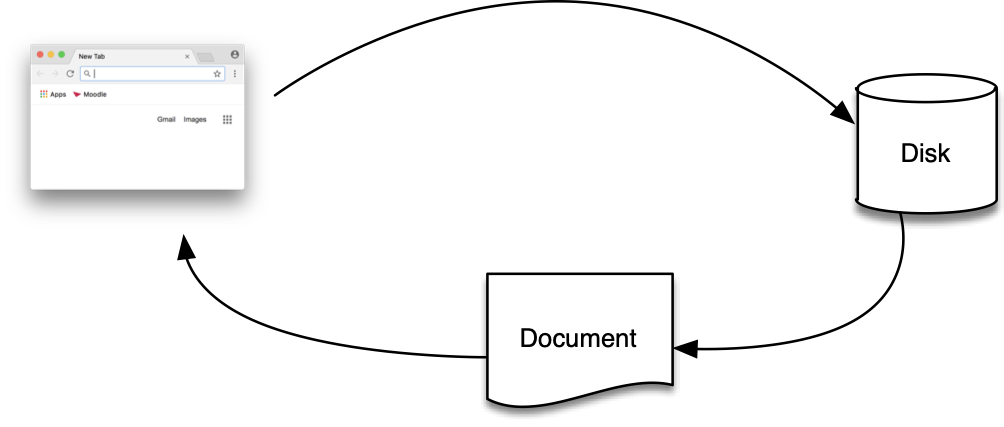
\includegraphics[width=0.8\textwidth]{figures/local-web-dev}
\label{fig:local-web-dev}
\caption{}
\end{figure}

\paragraph{} This is definitely using web technologies, but the resulting site is not part of the Web. This is because the site hasn't yet been deployed or published.


\section{Deployment}
\paragraph{} In order for our site to be available on the web, we need to store our web pages where they are accessible to our users. For our sites to be accessible we mean that a client (other than ourselves on our local machine) can connect to the storage location and request specific pages and "use the site". Note that there are other meanings of the term "accessible", usually in the context of the accessibility of the site, how usable the site is for different categories of user, but we'll leave that aspect to one side for now. The accessible location is known as a server, or more strictly, a web server. Note again, that the term "server" is overloaded terminology: server can refer to a hardware server, or a software server but can also refer to different types of software, for example a web server or a database server amongst many other types of software server. For our purposes, when we refer to a server in this unit we are referring to a web server.
\paragraph{} We could install web server software on our local machine and then go through the process of exposing that web server to the wider world but that raises many issues about security and requires lots of administrative skills that we haven't considered so far in this module and which are a bit out of scope. That said, you should definitely, at some point, consider trying to deploy a web server so that you understand the process of turning a regular computer into a web server. For the rest of this unit though we are going to consider using third party services and hosting providers.

\section{Server Hardware}
\paragraph{} A hardware server is a computer that is connected to a network, usually the Internet and which is running server software. There are many kinds of server software but we're only concerned with web server software for now. The hardware server accepts connections from other Internet users (often called clients) and then performs the tasks specific to the kind of server software it is running.
\paragraph{} Hardware servers can be basically any computer, from a Raspberry Pi right through to huge clusters, mainframes, and supercomputers, and including nearly everything in-between. Note also that a Raspberry Pi is not the minimal computer required to run a web server. Many Internet of Things (IoT) devices run tiny web server software to provide user interfaces to their owners for configuration.


\section{Server Software}
\paragraph{} Server software runs on a computer. Conveniently, the act of running server software turns the hosting hardware into a hardware server by extension. Server software listens for incoming connections and then responds appropriately to those connections.
\paragraph{} For the Web, server software is usually, primarily, HTTP server software. This is merely a piece of software that implements the HTTP protocol so that:

\begin{enumerate}
\item It can listen for incoming HTTP requests, and can
\item Respond appropriately to those requests by sending responses.
\end{enumerate}

\paragraph{} There are lots of implementations of HTTP Server Software, including:

\begin{itemize}
\item NGinX, 
\item Apache, 
\item IIS, 
\item Lighttpd (``lighty'')
\end{itemize}

\paragraph{} Installation and maintenance of HTTP/Web server software is usually the domain of system administrators rather than developers but you should still have some awareness of what happens after your site is designed and built, the process of making your site available on the Web.
\paragraph{} As a rule, an HTTP server needs to be connected to the Internet and have a valid, reachable IP address. The server listens for connections. The default port for web connections is port 80. This is so common that browsers connect automatically to port 80 when you type in a web address. Web servers can also listen on any other valid port from the range of 65536 available ports on each hardware server. Many of these ports though are generally reserved for services other than the Web. A secondary standard web port is port 8080 which you might occasionally see in the wild, usually because it is specified in the web address of a given site.

\section{Clients \& Servers}
\paragraph{} The ``Client/Server Architecture'' is a long established approach for organising communication between different devices and also between different pieces of software. Client/Server Architectures are used in lots of places in computing but we’ll assume from now on that we are dealing solely with HTTP servers.
\paragraph{} With an HTTP server, a client makes a request to a specific server (using a web address to identify which one). The server is already listening for requests. When a request is received the server determines what to do according to the HTTP protocol which specifies the allowed responses. The server then sends an appropriate message back to the client. That constitutes a single request-response cycle. The client can subsequently initiate additional communications by sending new requests.
\paragraph{} Note that this relationship of  client initiating a request and the server responding is fairly standard, unless you’re using the XWindow system in which case the relationship is back to front.

\begin{figure}[H]
\centering
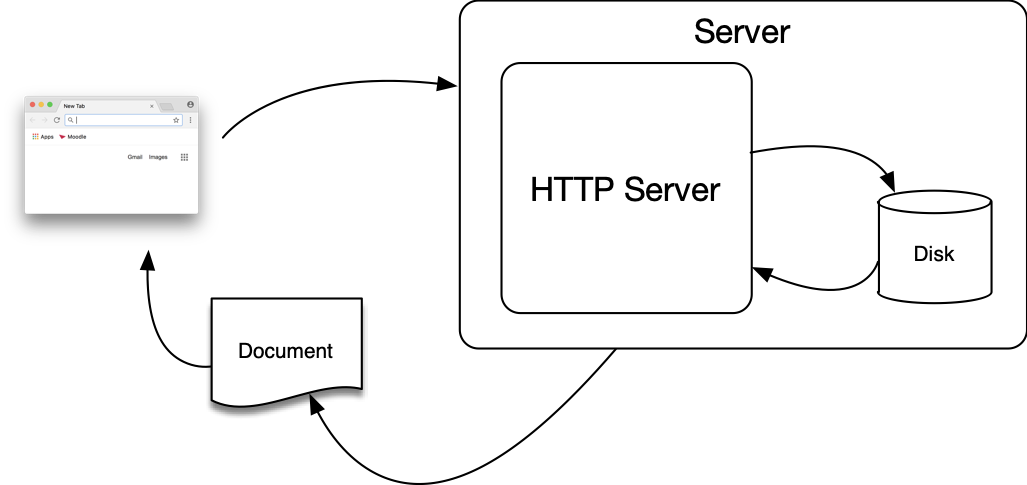
\includegraphics[width=0.8\textwidth]{figures/client-server}
\label{fig:client-server}
\caption{}
\end{figure}


\paragraph{} The server is a nexus. Multiple clients can connect to it with their own individual requests and the server will respond appropriately within the rules set down by the communication protocol.


\section{HyperText Transfer Protocol (HTTP)}
\paragraph{} The HyperText Transfer Protocol (HTTP) is a formal definition of how web servers and web clients can interact. It defines how (primarily text) messages for transferring HyperText should be:

\begin{itemize}
\item formatted and transmitted
\item responded to by servers and clients upon receipt of a given message
\end{itemize}

\paragraph{} HTTP is a core standard of the Web along with HTML. The relationship between the two is straightforward, HTML defines how to structure and inter-link web documents and HTTP defines how to move those web documents around so that they can be read and their links navigated.

\paragraph{} Technically, HTTP is a stateless, application layer protocol for communicating information between distributed systems.


\section{Deploying our own sites}

\paragraph{} We have a number of options when it comes to deploying our web sites. We can:

\begin{itemize}
\item Run a Local web server on our development machine. 
\item Use a free static hosting service. 
\item Use a Dedicated Web hosting service
\item Use a Virtual Server
\item Use a Hardware Server
\item Use a Cloud Host
\end{itemize}

\paragraph{} We'll now consider each in turn...

\subsection{Local Web Server}
\paragraph{} This is not really deployment but can be useful when developing a web site. It means that we can get our site to act during development as if it was publicly hosted. This can occasionally help us to identify some bugs that are only obvious after deployment. Note that there are also browser functionality limitations as a result of the browser security model which limits what a browser can do when reading files from the local file system, so running a local web server is useful when you run into these limitations.
\paragraph{} To run a local web server you should choose some appropriate software. NginX is a good choice, install and run NGinX (or another web server) locally on your development machine then connect to that local web server using the localhost or 127.0.0.1 address, accessing whichever port was set up by default for your installed web server (usually port 80 or 8080 but can be other ports).
\paragraph{} This is good for testing your sites and helps answer questions like: does my site behave the way it is supposed to when served up by a server? Do the links on my site work correctly?
\paragraph{} A local web server can be made available to other Internet users (but this gets complicated fast and is outside of the scope of this module).


\subsection{Free Static Hosting}
\paragraph{} There are many free static hosting services out there on the Web. These are sites that provide you with free web space for hosting and serving reasonably simple sites. These usually restrict you to plain HTML, CSS, and JS pages and have very limited, if any, server side dynamic functionality.
\paragraph{} Github Pages\footnote{\url{https://pages.github.com/}} is one such hosting service, albeit really oriented towards the needs of the open-source software community. This includes static hosting direct from your GitHub repository. When you push updates to your Git repository in GitHub the changes to your site are automatically deployed and made available to all web users. We've already seen how to deploy to GitHub pages during earlier lab activities. For more information visit:
\paragraph{} NeoCities\footnote{\url{https://neocities.org/}} is another free hosting service where you can deploy your static sites. This is an "old School" style of free, static site hosting which has been designed to be reminiscent of the Web of the 1990s. It is named for an older web host service called Geocities (which is, incidentally, where I published my own first ever website back in 1998). For more information visit:
\paragraph{} There are many free static hosting providers. Both GitHub Pages and Neocities have been around for a while but the hosting eco-system is very dynamic and you should investigate what is currently available should you want to try something different. You should also be aware that many of the commercial hosting providers also offer free-tiers amongst their services which can give you similar free, high-quality hosting for smaller sites.

\section{Dedicated Web Hosting}
\paragraph{} Many sites provide web hosting for a price. Often such hosters provide additional features and guarantees which can be useful if the site that you are deploying is important.
\paragraph{} The process is generally as follows:

\begin{itemize}
\item Sign up for an account, 
\item Pay the fees (start small/sometimes free) escalate rapidly depending upon bandwidth/features
\item Upload your pages
\end{itemize}

\paragraph{} There is often some limited control over the specific web server software and frequently some additional choices of pre-packaged “web” tools for deploying Wordpress, Joomla, \&c. Although out of scope for our purposes right now, these providers can also sometimes offer limited server-side dynamic hosting as well.

\paragraph{} Amongst the providers in this sphere are 1\&1 Ionos, RackSpace, Fasthosts, and many, many more…

\subsection{Virtual Server}
\paragraph{} This option gives you a complete virtual machine on someone else’s hardware server. This is connected to the Internet and you will pay for CPU, RAM, Storage, and bandwidth, according to your needs. This can start very cheap. There are some free virtual server hosts which offer their lower priced virtual servers from ~£2.99/month but prices can escalate very rapidly.
\paragraph{} A virtual server is basically a complete remote computer and you will often get a basic install of a Linux machine (although some hosts support other operating systems). You get almost complete control over your machine, but now have to assume much more of the administration of your machine and its operating system. You will usually start with a basic Linux machine and must build up the software side of your server from there, installing all software, languages, web servers, databases, etc. as needed.
\paragraph{} It is usually easy to backup and move your server to other places and gives you flexibility, perhaps to keep an ``in house'' clone of your virtual server locally for development and offline testing.
\paragraph{} Again there are plenty of providers available and the market is quite dynamic. Currently providers include the following: Fasthosts, 1\&1 Ionos, Digital Ocean, Linode, and OVH.
\paragraph{} A virtual server is a good and useful middle ground for more dynamic sites or ones where you need to exert more control over the way that you site is served and administered. You can easily scale up by purchasing a virtual server from a higher tier e.g. more RAM, CPU, Storage, Bandwidth, etc depending upon your needs. This is often possible with minimal effort and simple reboot.


\subsection{Hardware Server}
\paragraph{} One of the more expensive, but perhaps most flexible solutions for web hosting is your own hardware server. This is an actual physical machine, located in your own premises or in a hardware hosting facility. This is Hardware that you build, buy or rent. It must be connected to the Internet and this connection needs to be through a reliable network with a dedicated IP address.
\paragraph{} All administration must be done by you or others in your team. You must still build up the server software installation just like with a virtual server. You must also consider back-up and have a plan for expansion if your server can't keep up with the popularity of your site.


\subsection{Cloud Host}
\paragraph{} Cloud Hosting is sometimes a fancy name for a virtual server but can also refer to the idea of “computing as a service” and the provision of "Web services". Again, there are many options for web service based cloud hosts, Amazon Web Services and Google Cloud Computing are two of the biggest providers.
\paragraph{} Cloud hosting is scalable to the degree that you can afford and offers great flexibility but, especially at the more expensive end, the balance of advantages and disadvantages between a cloud hosted environment and a hardware setup can change and it can become cost-effective to manage your own infrastructure once more.
\paragraph{} Ultimately though, you should remember that a cloud machine is basically, someone else’s computer, with the attendant security and privacy issues associated with that. Note that this also affects all types of hosting. Before choosing a host, and definitely before deploying your site you should be considering where the server is located and also the associated legal jurisdiction. Does this have any effect on the type of site you intend to deploy? Whilst the Web is global, the machines that provide the functionality for the Web are still physically located somewhere in the world and are thus beholden to the laws that pertain in that location.

\section{Web Standards}
\paragraph{} Now let's take a final detour to consider web standards. These are the publicly agreed documents that underpin the Web. They define the protocols, like HTTP, and they define the languages, like HTML5, and CSS3, of the Web.
\paragraph{} Part of the success of the web is due to the goal of enabling non-experts to publish to the web. Clients and servers are quite relaxed about what they will accept, for example, HTML can be quite malformed before it becomes un-displayable. Usually we will still get the text content displayed as the most basic fall back. A major part of the success of the Web stems strongly from the existence of basic agreements on how all the parts work together. There are written agreements (standards) that describe these agreements. There are bodies (groups of people and organisations) that engage in multi-year negotiations to design and document standards for how the Web works. The role of these bodies is  usually to develop new standards (to govern new circumstances) or enhancing existing standards (because we rarely get anything perfect the first time around).
\paragraph{} There are three important bodies involved in standardising the web. These are:

\begin{itemize}
\item The Internet Engineering Taskforce (IETF)
\item The World Wide Web Consortium (W3C)
\item The Web Hypertext Application Technology Working Group (WHATWG)
\end{itemize}


\section{The Internet Engineering Task Force (IETF)}
\paragraph{} The Internet Engineering Task Force (IETF) is an organisation who develop and promote open standards for the Internet. Whilst this isn't focused specifically on the Web, the Internet underpins most of the functionality of the Web, so what happens with respect to Internet protocols is of huge importance.
\paragraph{} The IETF is primarily known for the TCP and IP standards. These are:

\begin{itemize}
\item TCP - The Transmission Control Protocol. A protocol for transmitting packets of data between computers.
\item IP - The Internet Protocol. A protocol for uniquely addressing machines on the Internet (hosts) and enabling them to find each other.
\end{itemize}

\paragraph{} The IETF also defines the standard for HTTP (HyperText Transfer Protocol) so is an important organisation from the Web perspective. 
\paragraph{} In summary the IETF controls how computers find each other (addressing), how computers move data between each other(transmission), and how a hypertext system can be built on top of a system that already offers both addressing and transmission.
\paragraph{} Note that all of these layers could be replaced with different approaches. No single layer is necessary in the form that it currently exists and each will be enhanced, and possibly replaced, over time. 
\paragraph{} The surface features of the Internet and Web stem from the aggregation of these underlying standards providing sufficient functionality for higher level needs, like transmitting HTML from a server to a browser, but other approaches could be taken, i.e. using different addressing protocols or different transmission protocols.

\section{The World Wide Web Consortium (W3C)}

\paragraph{} The World Wide Web Consortium (W3C) is another international standards organisation, like the IETF. This time though the focus is on the needs of the Web specifically rather than the wider Internet. The W3C has traditionally taken a quite conservative and unwieldy approach to standardisation. The standardisation process involves multiple stages:

\begin{itemize}
\item Working Draft - After discussion of ideas a WD is published for review. Can implement WD standards but likely to be huge future changes
\item Candidate Recommendation - When standard meets initial design goals the wider community is solicited to feedback on practicality of implementation
\item Proposed Recommendation - Having passed through WD and CD stages a PR is put to the W3C advisory council for approval
\item W3C Recommendation - A standard that has been endorsed by W3C membership after extensive development, testing, and evaluation
\item Revisions - Updates or extensions published until sufficient for new edition of the standard
\end{itemize}

\section{The Web Hypertext Application Technology Working Group (WHATWG)}
\paragraph{} The Web Hypertext Application Technology Working Group (WHATWG) was established in 2004 as a response to the slow pace of development of W3C web standards. Primarily the decision by W3C to focus on XML-based technologies instead of HTML was seen as a mis-step by many. Web developers are famously pragmatic and XML introduced huge complications without obvious immediate benefits. Thus the WHATWG was born to work around the W3C. The central and steering members include: Apple, Mozilla, Google, and Microsoft, so some of the biggest commercial organisations in computing and technology. However contributors to the WHATWG can be anyone who joins the WHATWG mailing list.
\paragraph{} The WHATWG focus is upon the following:

\begin{itemize}
\item The HTML Living Standard. This is essentially the development of HTML 5 and beyond. HTML 4 is now adopted by W3C as the starting point for new HTML development. The notion of a living standard means that rather than a single, defined standard, the move is now towards continuous changes as the Web, and the way it is used, evolves. The living standard also incorporates additional APIs beyond pure HTML, e.g. WebSocket, WebWorker, LocalStorage, etc.
\item DOM standard — defining how the Document Object Model works so that all browsers can operate to a shared model.
\item Fetch standard — defining requests and responses and the process that unifies them so that there can be a single agreed way to access remote APIs from a browser instead of using XMLHTTPRequest or some other similar hack.
\item Plus a whole host of additional ancillary standards including the web worker API, Microdata vocabularies, storage API standards, data streaming API standards, Encoding standards (e.g. UTF-8), MIME-type sniffing, URL parsing standards.
\end{itemize}

PThere are some benefits to having the WHATWG in addition to the W3C. The WHATWG assumes some responsibilities that the IETF has traditionally worked on alone, e.g. URL standards, HTTP standards by replacing RFCs with WHATWG living standards. The aim is to assume responsibility for developing standards more rapidly and pragmatically and this has led to improvement. The disastrous direction of HTML during the XHTML years has been addressed, replacing the complex HTML4 standard with a streamlined, focused, and more understandable HTML 5 standard.


\section{Summary}
\paragraph{} We've now completed our survey of client-side web technologies by considering how to deploy our websites so that they can be found by Web users. During this process we've looked at moving from local development to web development. We’ve investigated servers and clients, and how these relate to Web servers and the HTTP protocol. We’ve also considered the various options for deploying our websites, from free hosting through to more expensive cloud hosting. Finally, we introduced the three important organisations that set the standards which underpin the Internet and the Web. Without these organisations there wouldn't be the agreements that enable the Web to work the way it does. As your career will probably outlast the current Web standards, it is well worth knowing to whom to turn to find out what new ideas and technologies are on the horizon.
